\documentclass[a4paper, 11pt]{article}
\usepackage[UTF8, scheme = plain]{ctex}
\usepackage{float}
\usepackage{amsmath}
\usepackage{graphicx}
\usepackage{geometry}
\usepackage{listings}
\geometry{scale=0.8}
\linespread{1.5}
\usepackage{hyperref}
\lstset{literate=
    {↑}{{$\uparrow$}}1
    {→}{{$\rightarrow$}}1
    {↓}{{$\downarrow$}}1
    {←}{{$\leftarrow$}}1
}

\title{	
\normalfont \normalsize
\textsc{School of Data and Compuaer Science, Sun Yat-sen University} \\ [25pt] %textsc small capital letters
\rule{\textwidth}{0.5pt} \\[0.4cm] % Thin top horizontal rule
\huge  HW3 Sarsa and Q-Learning\\ % The assignment title
\rule{\textwidth}{2pt} \\[0.5cm] % Thick bottom horizontal rule
\author{18308045 谷正阳}
\date{\normalsize\today}
}

\begin{document}
\maketitle
\tableofcontents
\newpage
\section{Cliff walk}

This gridworld example compares Sarsa and Qlearning,
highlighting the difference between on-policy (Sarsa) and off-policy (Qlearning) methods.
Consider the gridworld shown in the upper part of Figure 6.5.
This is a standard undiscounted, episodic task,
with start and goal states,
and the usual actions causing movement up, down, right, and left.
Reward is $\textnormal{-}1$ on all transitions except those into the region marked “The Cliff.”
Stepping into this region
incurs a reward of $\textnormal{-}100$ and sends the agent instantly back to the start.

\begin{figure}[H]
  \centering
  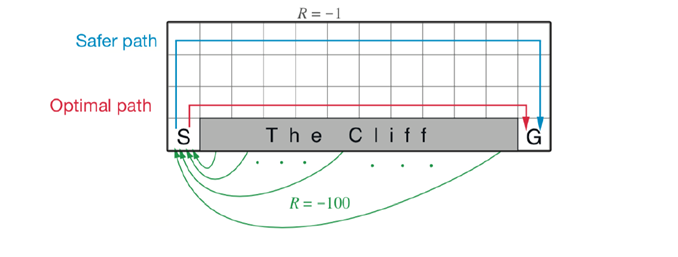
\includegraphics[width=16cm]{cliff_walk.png}
  \caption{Cliff walk}
\end{figure}

\section{Implementation of algorithm}

\subsection{$\epsilon$-greedy exploration}

$\epsilon$-greedy是$\epsilon$的概率以相同的概率选一个action,
$1-\epsilon$的概率选最优action。

$\epsilon$的概率用以下代码描述:

\begin{lstlisting}[frame=single,language=python,numbers=left]
random.random() <= epsilon
\end{lstlisting}

以相同的概率选用以下代码描述:

\begin{lstlisting}[frame=single,language=python,numbers=left]
action = random.choice(actions)
\end{lstlisting}

最优则直接调用greedy:

\begin{lstlisting}[frame=single,language=python,numbers=left]
greedy(actions, Q_state)
\end{lstlisting}

\subsection{Sarsa}

MC是用历史的episodes在各个state采取action的G均值来评估,
即对每个episode的每个state,action使用
$Q(S_t,A_t)\leftarrow Q(S_{t-1},A_{t-1})+\frac1{N(S_t,A_t)}(G_t-Q(S_{t-1},A_{t-1}))$,
使$Q(S_t,A_t)$一直是$G_1\cdots G_t$的平均值。

Sarsa是将上述公式用$Q(s_{t+1},A_{t+1})$
近似代替$G_{t+1}=R_{t+2}+\gamma R_{t+3}+\cdots$
即以$R_{t+1}+\gamma Q(S_{t+1},A_{t+1})$近似代替$G_t$,
使之可以不用等到全部episodes结束即可进行计算。

另外,为了简化计算,这里用running-mean来代替普通的均值,
即用常数$\alpha$代替$\frac1{N(S_t,A_t)}$。

代码体现如下:

\begin{lstlisting}[frame=single,language=python,numbers=left]
Q[state][action] = Q[state][action]\
    + alpha * (R + gamma * Q[state_new][action_new]
                - Q[state][action])
\end{lstlisting}

为了在没有exploring starts的情况下,仍能保证所有actions可以被选到,
使用$\epsilon$-greedy,即每个action被选的概率都不为0。体现如下:

\begin{lstlisting}[frame=single,language=python,numbers=left]
action_new = epsilon_greedy(puzzle.get_actions(),
                            Q[state_new], epsilon)
\end{lstlisting}

\subsection{Q-Learning}

Q-Learning是一种off-policy learning,在sarsa的基础上,使用了两种policies。
一种是更有探索性的behavior policy即当前使用$\epsilon$-greedy,体现如下:
\begin{lstlisting}[frame=single,language=python,numbers=left]
action = \
    epsilon_greedy(puzzle.get_actions(), Q[state], epsilon)
\end{lstlisting}
另一种是学习用来选最优action的target policy即假设下一步使用greedy,体现如下:
其好处有很多,如既可以保证探索性,又可以保证最优。
可以证明其最终两个policies都收敛。
算法体现如下:
\begin{lstlisting}[frame=single,language=python,numbers=left]
action_new = greedy(puzzle.get_actions(), Q[state_new])
\end{lstlisting}

\subsection{Ploting}

绘制run\_times次总rewards的均值,参数设置如下:

\begin{lstlisting}[frame=single,language=python,numbers=left]
num_episodes = 500
range_num_episodes = range(num_episodes)
alpha = 0.5
gamma = 1
epsilon = 0.001
run_times = 20
\end{lstlisting}

\section{Results}

\subsection{Figure}

\begin{figure}[H]
  \centering
  
\includegraphics[width=18cm]{result.png}
  \caption{Result}
\end{figure}

\subsection{Terminal}

篇幅受限,请见附件result.txt。

%\clearpage
%\bibliography{E:/Papers/LiuLab}
%\bibliographystyle{apalike}
\end{document} 
%%% Local Variables:
%%% mode: latex
%%% TeX-master: t
%%% End:
